\chapter{Formakuntza saioa}\label{cha:formakuntza}

Behin formakuntza saioa oinarritzen den marko teorikoa osatuta, ondorengo atalean, honen diseinua gauzatzen da. 

\section{Formakuntzaren aurkezpena}\label{hemendik aurrera ez dao labek gehixau, pereza maxima}

Praktika Komunitate Profesionalen markoan oinarritutako formakuntza saio hau, esparru publikoko, DBH eta Batxilergoko irakasleei zuzendua dago, Informazio eta Komunikazio Teknologien (IKT) irakaskuntza modu zuzen batean etapa horietan lantzen delako gehienbat. Formakuntza honekin lortu nahi dena, ikastetxeetan erabiltzen diren baliabide digitalen irakurketa kritiko bat egitea da, inguratzen dituzten elementuen ondorioen jakitun izateko. Baita ere, burujabetza digitalaren filosofia ezagutaraztea eta horretan lanean dauden eragile/elkarteak aditzera ematea eta hauek proposatzen dituzten erabilera libreko softwareetan irakasleak trebatzea, ondoren jakintza eta lan egiteko modu hauek ikasgeletan transmititzeko. 

Formakuntza hau 5 saio nagusitan antolatua dago, bakoitza 2-3 orduko iraupena dutenak. Saioak hilabeteko lehen astelehenetan izango dira. Modu honetara, saio bakoitzetik bestera hilabeteko tartea egongo da ikasitako edukiak ikastetxean aplikatzen hasteko eta aldi berean denbora tarte horretan emandako bilakaeraren balorazio bat egiteko. Bertan, metodologia aktiboak erabiliz talde eta banakako lanketa, hausnarketa eta dinamikak eramango dira aurrera.

Edukien aipamen bat egitearren, lehen saioan GAFAM enpresek hezkuntzan aurrera eramaten duten eskuhartzea landuko da. Bigarrenean, burujabetza digitalaren kontzeptuan sakonduko da, horretan lanean dauden elkarteak ezagutaraziz eta hainbat adibide konkretu ikusiz. Hirugarren formakuntzan, software libreen gaian sakonduko da, zer diren, zertan oinarritzen diren eta non aurki daitezkeen azalduz eta laugarren saioan, hauetan trebatzea izango da asmoa. Azkeneko saioan, hausnarketa eta ebaluaziorako tartea irekiko da.

\section{Helburuak}

Formakuntzaren helburu nagusia, gaur egun ikastetxeetan ematen den digitalizazio prozesuaren bilakaeraren aurrean irakasleak hausnarketa kritikora bultzatzea. Digitalizazio prozesu honen norantza ikusita, burujabetza digitalerako bidean urratsak emateko asmoz, baliabide digital libreetan trebatuko dira saio hauetan zehar.

Helburu nagusia betetzeko bidean, hainbat helburu espezifiko definitu dira, formakuntzan zehar landuko diren edukiekin lotura zuzena dutenak:
\begin{itemize}
    \item Hezkuntza mundura hurbildu eta geratzeko etorri diren GAFAM enpresa multinazionalen ekosistema digitalak ikastetxeetan txertatzeko asmoak ezagutzea eta EAEko hezkuntza sistemaren eta gure ikasleen eskubideak urratzeak duen eraginaz ohartu eta hausnartzea.
    \item Egungo hezkuntza sisteman GAFAM enpresen esku hartzeari aurre eginez eta burujabetza digitalera bidean alternatibak planteatuz lan egiten duten eragile eta proiektuak ezagutarazi eta hauek aurkezten dituzten proposamenen inguruan hausnartu.
    \item Gaitasun eta trebeziak lortzetik haratago, irakaslea teknologia digitaletan ahalduntzea. Horretarako, hezkuntzan erabiltzen diren baliabide digitalak zerrendatzea eta hauetan enpresen eskuhartzea identifikatzea. Baliabide alternatibo libreak aurkitzea eta aurkitzen jakitea (burujabetza garatzea). Alternatiba nagusien erabileran trebatzea.
    \item Saioen artean definitutako helburuetan fokua jarriz, irakasle mintegiko kideen artean jakintzak partekatzea, komunitate profesional bat eratzen joanez eta aldi berean, emandako aurrera pausuen gaineko balorazioak eginez.
    \item Hezkuntza curriculumean bildutako KDen harira, garatutako kontzientzia hau ikasleen formakuntzan islatzea, baliabide digitalak erabiltzerakoan, hausnarketa hauetara itzuliz.
\end{itemize}

Helburu hauek lortzeko, formakuntza saioan landuko diren edukiak finkatuko dira jarraian. Eduki hauek formakuntza saioaren hiru ardatzetara orientatuta joango dira.

\newpage
\section{Edukiak}

Formakuntza saio honetan, 3 ardatz bereizi daitezke. Alde batetik, hezkuntza munduan esku hartzen duten enpresa pribatuen ezaugarritzea egingo da. Ondoren, enpresa hauen eskuhartzea murrizteko dauden joerak ezagutuko dira. Azkenik, joera horiek oinarritzen diren tresna libreetan trebezia garatuko da.

\begin{enumerate}
    \item Hezkuntza sisteman esku hartzen duten enpresen ezaugarritzea.
    \begin{enumerate}
        \item GAFAM enpresak ezagutu.
        \item GAFAM enpresen eskuhartzea eta bilakaera hezkuntzan.
        \item Multinazional hauen azaleko zein ezkutuko helburuak ezagutu, hezkuntza sistemari dagokionez.
        \item EAEko hezkuntza sistemako panoramaren diagnosia GAFAM enpresekiko
        \item Ikastetxeetara hurbilpena eta ikaslean fokua jarriz egungo egoeraren hausnarketa kritikoa garatu.
\end{enumerate}
    \item Hezkuntzako eredu digitalari aurre egiten dioten planteamenduen ezaugarritzea eta hauen jarduna EAEn.
    \begin{enumerate}
        \item Burujabetza digitalaren ideia ezaugarritu.
        \item Mugimendu horretan lanean dauden elkarte eta eragileak ezagutu eta hauen bilakaera aztertu (bertakoak eta atzerrikoak).
        \item EAEn aurretik eramandako proiektu/lan/aurrera-pausuak arakatu.
        \item Ikastetxeko azpiegitura digitalaren diagnosia definitu burujabetza mailarekiko.
\end{enumerate}
    \item Hezkuntzaren arlo digitalaren pribatizaziorako joeraren aurkako tresna eta baliabideak eskuratu.
    \begin{enumerate}
        \item Baliabide digitalen jatorria aztertzen jakin, erabiltzen diren baliabideak identifikatu.
        \item Alternatiba libreak ezagutu eta erabiltzeko joera bultzatu.
        \item Tresna pribatiboak erabiltzeko unean, izaera kritikoa landu.
        \item Software libretik datorren ideologia transmititu.
        \item Tresna erabilgarrietan trebatu, aldaketara pausua ematera bultzatu. 
        \item Irakaskuntza komunitatean tresna hauek zabaldu.
\end{enumerate}
\end{enumerate}


\section{Metodologia}

Hilabeteko tartea egongo denez saioen artean, garrantzitsua da jarraikortasuna bermatzea. Honetarako, aplikatuko den zentrotik arduradunak izendatuko dira, eta formazio guztira etorri beharko dira. Gogorarazi behar da formakuntza honen helburuetako bat PKPa eratzea dela, beraz arduradun hauek egunerokotasunean beste irakasleak komunitatean integratzeko betebehar batzuk izango dituzte. Hau ahalbidetzeko, irakaslegoaren \%40a bertaratzea espero da (20 irakaslerentzako prestatua dago formakuntza saioa), eta gutxienez departamentu bakoitzeko pertsona bat izatea lagungarria izan daiteke.

Lehenengo saio eta bigarren saioaren amaieran behaketa taulak sortuko dira, ikastetxearen diagnosia egiteko. Behaketa taula hauek saio bakoitzeko teoriarekin beteko dira, eta ikastetxearekiko izaera kritikoa izango dute. Hurrengo hilabeteko saioaren hasieran, behaketa taula aztertu eta ondorioak aterako dira, eta saio bakoitza ondorio hauetatik hasita birbideratuko da.

Hirugarren saioaren amaieran, ikastetxean egin daitezkeen aldaketa batzuk proposatuko dira. Ez du zertan errealista izan behar, laugarren saioan hausnartu eta epe luzerako plangintza bat finkatzeko balio izango du eta. Epe luzerako plangintzaren muina ikastetxe librezalearen kultura sortzea izango da.

Honetaz gain, DigCompEdu markoan oinarrituta, irakasleen hasierako konpetentzia digitalak neurtuko dira. Horretarako, eskaintzen den formularioa beteko da eta baliagarria izango da formazioan zehar maila altuena duten irakasleak IKTko arduradun bezala izendatuak izateko. Prozesu honetan zehar sortu daitezkeen zalantzak arduradun hauei komunikatuko zaizkie, eta hauek izango dira laguntzaile lana egingo dutenak (jakitun batekin kontaktuan jarriz edo beraien kabuz informazioa bilatuz).

Taldekatzerako orduan, pertsonen digitalizazio maila kontutan izango da. Aberasgarriagoa izan daiteke maila desberdinetako irakasleak elkarlanean aritzea, baina taldean DigCompEdu markoan “lider” rola duten irakasleak izateak gauzak erraztu ditzake. Hau dela eta, talde orokorraz gain, lau pertsonako “talde txikiak” sortuko dira, dinamiketan zehar erabiliko direnak.

\section{Denboralizazioa}

Irakasleei bideratutako formakuntza saio hau denboran zehar \ref{tab:plangintza} taulan ikusten den moduan antolatu da. 5 atal nagusiz osatua dago, eta atal bakoitza hilabeteko lehen astelehenetan burutuko da, honako gai desberdinak landuz. Irailetik aurrera hasiko da, ikasturtean zehar duen eraginaren gogoeta bultzatu nahi da eta.

\begin{center}
    \captionof{table}{\textit{Formakuntza saioaren plangintza}}
    \label{tab:plangintza}
    \begin{tabular}{|p{4,75cm}|p{9cm}|}
        \hline
        \rowcolor[HTML]{D9D9D9} 
        \textbf{DENBORALIZAZIOA} & \textbf{GAITEGIA}
        \\ \hline
        IRAILA → 1.saioa & GAFAM enpresen esku-hartzea hezkuntzan
        \\ \hline
        URRIA → 2. saioa & Burujabetza digitala, bide horretan lan egiten duten elkarteak eta hauen   proiektuak.
        \\ \hline
        AZAROA → 3. saioa & Tresna digital alternatiboak aurkitzen trebatu
        \\ \hline
        ABENDUA → 4. saioa & Baliabide digital libreetan trebatu
        \\ \hline
        URTARRILA → 5. saioa & Autoebaluazioa eta formakuntzaren ebaluazioa
        \\ \hline
    \end{tabular}
\end{center}

Saio bakoitzak 2-3 ordu bitarteko iraupena izango du eta saio bakoitzetik bestera hilabete bateko tartea egongo da. Formakuntza antolatzeko modu honen arrazoi nagusia saio bakoitzean eskuratutako ezagutzak ondoren ikastetxean lurreratzeko denbora edukitzea da, hau da, beste irakasleei ezagutza hauek transmititzea eta arlo honen progresurako bide orri bat diseinatzea beharrezko eztabaidak emanez. Gainera, lehen eta bigarren formakuntzetan behaketa taula ezberdinak prestatuko dituzte ondorengo hilabetean ikastetxeko egoera aztertzeko. Beraz, horretarako ere denbora behar da.

Horrez gain, behaketa taulako edukiak eta bertatik ateratako ondorioak mahaigaineratu eta horien inguruan hausnartzeko tarteak irekiko dira, taula osatu eta hurrengo formakuntza saioan partekatu eta talde gogoetak egin ahal izateko. Azken finean formakuntza saio guztiek elkarren artean lotura dute eta taula horietako edukia ezinbestekoa da ondorengo saioetarako oinarri moduan.

Jarraian, \ref{tab:denboralizazioa}. taulan, saio bakoitzaren denboralizazioa aurkitu daiteke. Saio bakoitzak hainbat fase izango ditu, helburu desberdinekin. Fase bakoitzak, aldi berean, dinamika ugari izango ditu.

\newpage
\begin{center}
    \captionof{table}{\textit{Formakuntza saioaren denboralizazioa}}
    \label{tab:denboralizazioa}
    \begin{tabular}{|p{3cm}|p{3cm}|p{3cm}|p{3cm}|p{3cm}|}
        \hline
        \rowcolor[HTML]{D9D9D9} 
        \textbf{1. SAIOA} & \textbf{2. SAIOA} & \textbf{3. SAIOA} & \textbf{4. SAIOA} & \textbf{5. SAIOA}
        \\ \hline
        \makecell{\textbf{0. Fasea:}\\
        Dinamika I:\\(15 min.)\\
        Dinamika II:\\(5 min.)} & 
        \makecell{\textbf{4. Fasea:}\\
        Dinamika IX:\\(10 min.)\\
        Dinamika X:\\(30 min.)} & 
        \makecell{\textbf{7. Fasea:}\\
        Dinamika XV:\\(10 min)\\
        Dinamika XVI:\\(20 min.)} &
        \makecell{\textbf{10. Fasea:}\\
        Dinamika XXI:\\(10 min)\\
        Dinamika XXII:\\(20 min.)} & 
        \makecell{\textbf{12. Fasea:}\\
        Dinamika XXV:\\(10 min)\\
        Dinamika XXVI:\\(30 min.)\\
        Dinamika XXVII\\(30 min.)}
        \\ \hline
        \makecell{\textbf{1.Fasea:}\\
        Dinamika III:\\(10 min.)\\
        Dinamika IV:\\(25 min)} &
        \makecell{\textbf{5. Fasea:}\\
        Dinamika XI:\\(30 min.)\\
        Dinamika XII:\\(25 min.)} &
        \makecell{\textbf{8. Fasea:}\\
        Dinamika XVII:\\(20 min.)\\
        Dinamika XVIII:\\(30 min)\\
        Dinamika XIX:\\(60 min.)} &
        \makecell{\textbf{11. Fasea:}\\
        Dinamika XXIII:\\(60 min.)\\
        Dinamika XXIV:\\(30 min.)} &
        \makecell{\textbf{13. Fasea:}\\
        Dinamika XXVIII:\\(40 min.)}
        \\ \hline
        \makecell{\textbf{2. Fasea:}\\
        Dinamika V:\\(20 min.)\\
        Dinamika VI:\\(45 min.)\\
        Dinamika VII:\\(30 min.)} &
        \makecell{\textbf{6. Fasea:}\\
        Dinamika XIII:\\(40 min.)\\
        Dinamika XIV:\\(40 min.)} &
        \makecell{\textbf{9. Fasea:}\\
        Dinamika XX:\\(20 min.)} &
        \cellcolor[HTML]{F2F2F2} &
        \cellcolor[HTML]{F2F2F2}
        \\ \hline
        \makecell{\textbf{3. Fasea:}\\
        Dinamika VIII:\\(40 min.)} &
        \cellcolor[HTML]{F2F2F2} &
        \cellcolor[HTML]{F2F2F2} &
        \cellcolor[HTML]{F2F2F2} &
        \cellcolor[HTML]{F2F2F2}
        \\ \hline
        \rowcolor[HTML]{D9D9D9}
        \multicolumn{5}{|l|}{\textbf{Saio bakoitzeko denbora totala}}
        \\ \hline
        3 h eta 10 min. & 2 h eta 55 min. & 2 h eta 20 min. & 2h. & 1h eta 50 min.
        \\ \hline
    \end{tabular}
\end{center}

\section{Baliabideak}

Formakuntza saio hau aurrera eramateko ezinbestekoa da hainbat material, fisiko zein digital, eskuragarri izatea.

\subsection{Baliabide fisikoak}

Baliabide fisikoei dagokienez, lehenik eta behin, ikasgela handi bat eskuragarri izatea beharrezkoa da formakuntza saioa aurrera eramateko. Hainbat talde dinamika eramango dira aurrera, beraz beharrezkoa da espazio zabal bat izatea, talde dinamiketan partaide guztiek tokia izateko. Bertan ondorengo materiala egon behar da:

\begin{itemize}
    \item Partaide guztiendako mahai eta aulkiak, mugitzeko errazak.
    \item Arbel zuria.
    \item Aurkezpenerako proiektore eta ordenagailu bat.
    \item Partaide guztiendako ordenagailuak (norberarenak).
    \item Zerbitzari bat.
    \item Dinamiketako taldeentzako baliabideak:
    \begin{itemize}
        \item Nota itsaskorrak.
        \item Boligrafoak.
        \item Orri zuriak.
        \item Arbelean idazteko boligrafoak.
    \end{itemize}
\end{itemize}

\subsection{Baliabide digitalak}

Baliabide digitalak ere behar-beharrezkoak izango dira formakuntzarako. Moodle plataforma bat sortu da, \url{http://burujabetzadigitala.eus/moodle/}-en eskuragarri. Bertan txertatu da formakuntzan zehar erabiliko den material guztia. Moodle plataformaren erabileraren inguruko informazio gehiago eskuragarri dago \ref{eranskin:moodle}-en.

Bertan, formakuntza saioko 5 egunetarako 5 kurtso desberdin aurki daitezke, eta aurkezpen moduan erabiliko den 0. saioa. Kurtso bakoitzak bere aurkezpena eta baliabideak ditu eskuragarri bertan. 5. saioa ebaluaketa saioa izango da, eta bertan hainbat ebaluaketa egiteko txantiloiak aurki daitezke.

Bukatzeko, kurtsoan zehar erabiliko diren hainbat baliabide digital zerrendatuko dira:

\begin{itemize}
    \item Baliabide irekiak:
    \begin{itemize}
        \item \href{https://es.libreoffice.org/}{LibreOffice} ofimatika kit-a.
        \item \href{https://www.mozilla.org/eu/firefox/}{Mozilla Firefox} nabigatzailea.
        \item \href{https://www.thunderbird.net/eu/}{Thunderbird} mail bezeroa.
        \item \href{https://duckduckgo.com/?kat=-1&kah=wt-wt&kad=eu_ES}{Duckduck Go} arakatzailea.
        \item \href{https://lubuntu.me/}{Lubuntu linux} sistema eragilea.
        \item \href{https://moodle.com/es/}{Moodle} ikasketa plataforma.
        \item \href{https://mailcow.email/}{Mailcow} eta \href{https://filezilla-project.org/}{Filezilla} zerbitzuak.
    \end{itemize}
    \item Baliabide pribatuak:
    \begin{itemize}
        \item \href{https://docs.google.com/forms/}{Google forms}.
        \item \href{https://kahoot.it/}{Kahoot!}.
        \item \href{https://youtube.com/}{YouTube}.
    \end{itemize}
\end{itemize}

Aipatu beharra dago, 4. saioa burutzeko ikastetxeko IKT arduradunarekin hitz egin behar dela, aurre prestakuntza bat beharrezkoa da eta. Hau burutzeko Moodlen bertan dago eskari horri bat, formakuntza planteatzerakoan bete beharko dena.

\section{Sekuentziazioa}
\captionof{table}{\textit{Formakuntza saioaren sekuentziazioa}}
\label{tab:sekuentziazio}

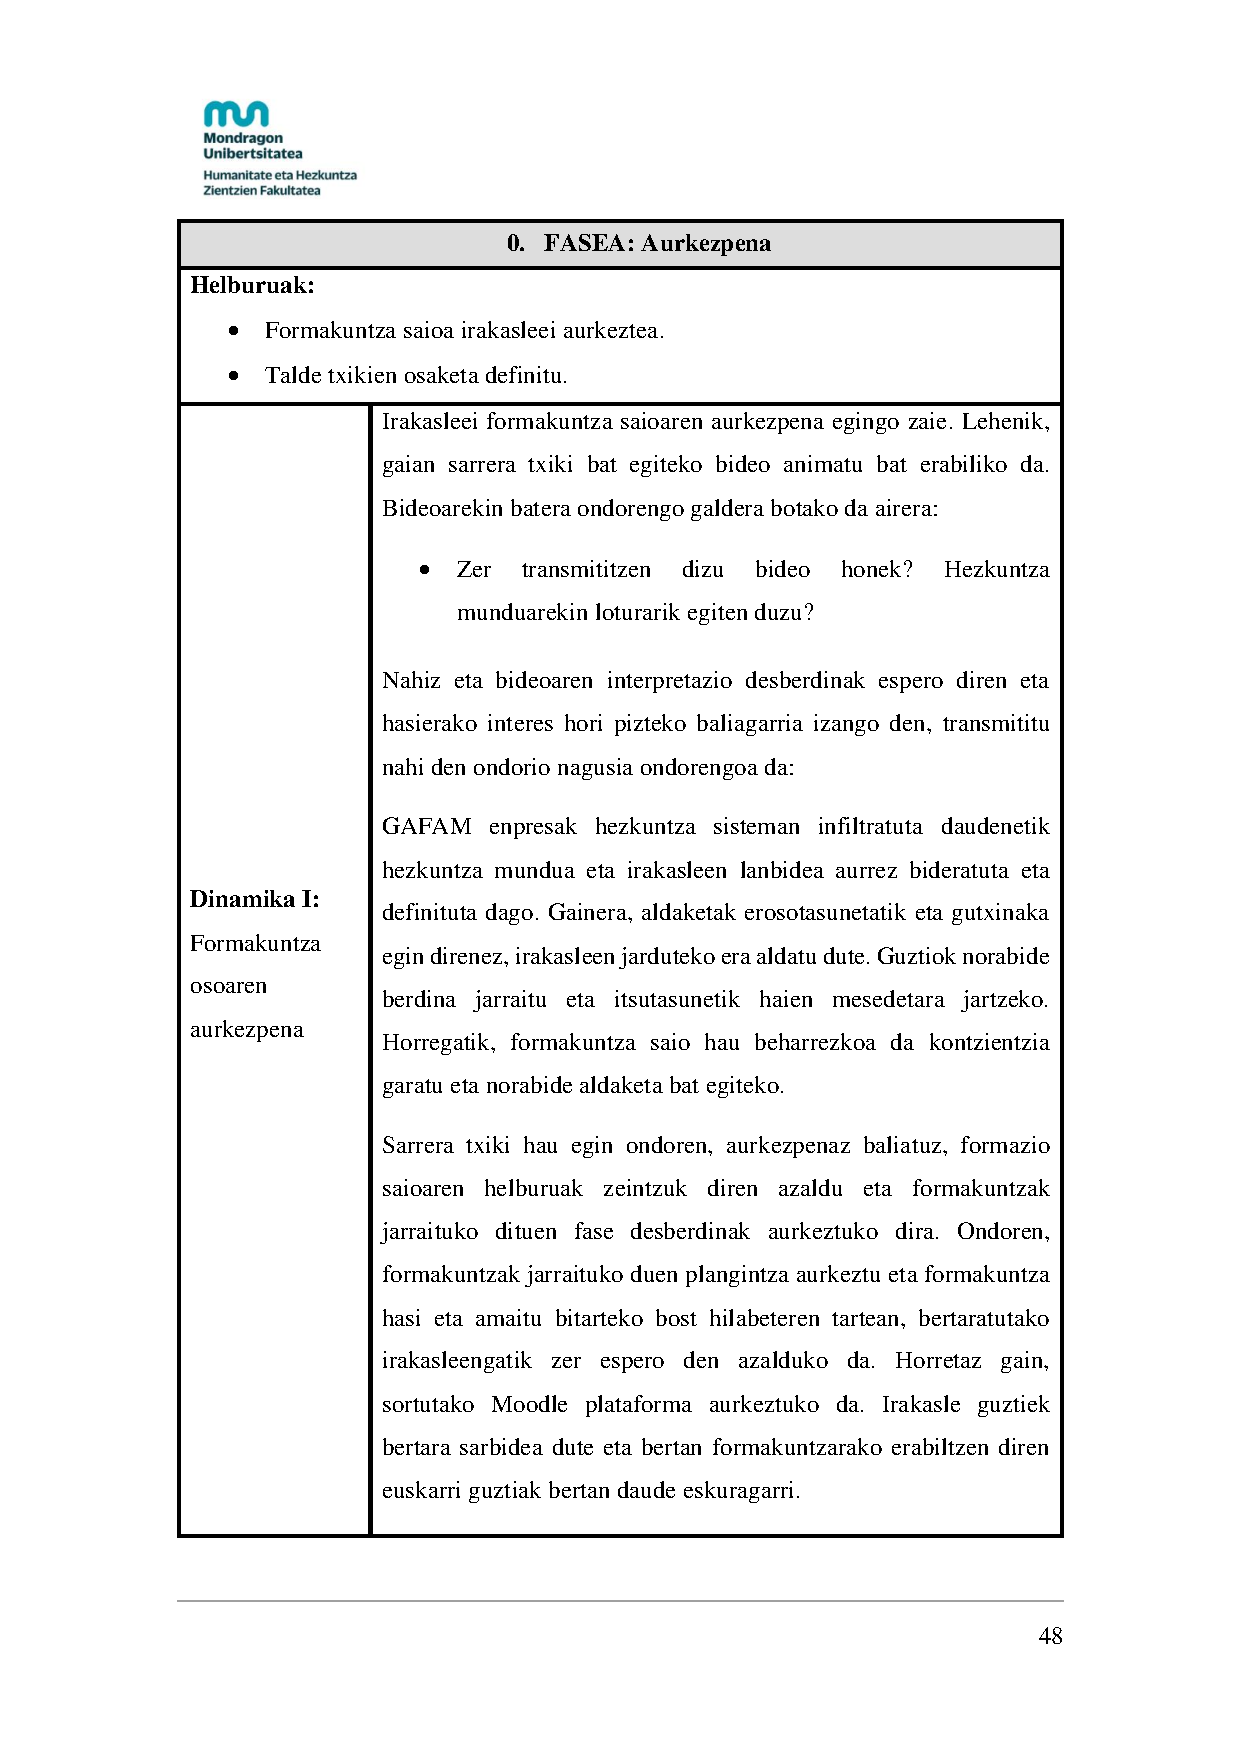
\includepdf[pages=-]{nnapa} %taula egiteko astirik ez dago

\section{Ebaluazioa}
Ebaluazioaren helburua, alde batetik formakuntza bera ebaluatzea da. Formakuntza bera eraginkorra eta dinamikoa izan den, baliabide egokiak erabili diren eta hobekuntzarako tarterik balego, ezaugarri hauek adieraztea da, besteak beste. Azken finean, ikastetxeetan eraginkorra eta baliagarria izango den formakuntza hau, formakuntza jasotzen duten irakasleen feedback eta hobetzekoekin osatzen joatea aberasgarria izango da partaide eta eragile guztientzat. 

Bestetik, formakuntza jasotzen duten irakasleek haien buruaren autoebaluazioa egitea litzateke bigarren helburua. Horretarako, formakuntzan jasotako baliabide eta hausnarketarako espazioak, irakasle jardunean eta gizarte honetako biztanle moduan izan duen eragina neurtzea. Hilabete hauetan zehar, hasierako eta amaierako egoerak kontuan hartuta, egindako prozesuaren kontzientzia hartu eta norberaren burua azaleratutako helburu eta gai desberdinekiko ebaluatzea eta kezkak adieraztea. 
